% Created by tikzDevice version 0.6.2-92-0ad2792 on 2013-10-13 05:46:33
% !TEX encoding = UTF-8 Unicode
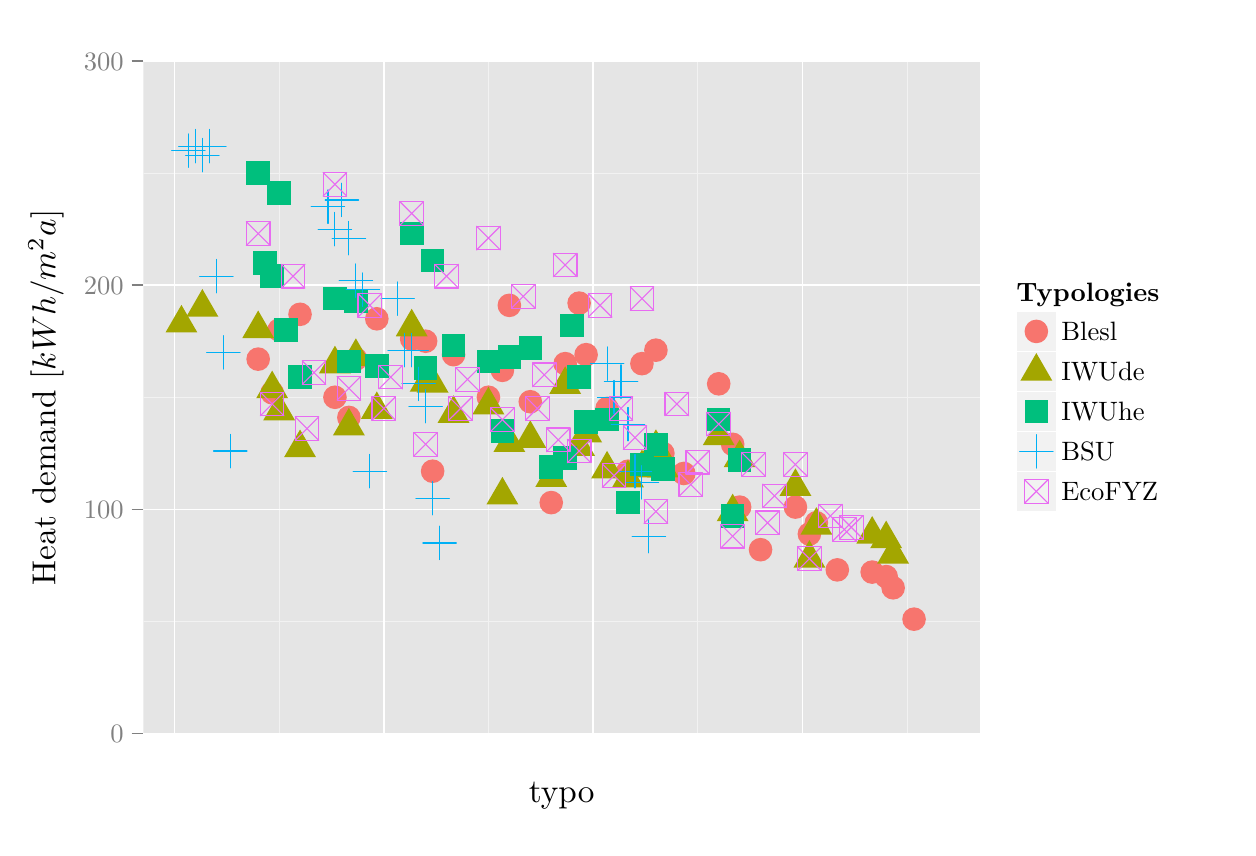
\begin{tikzpicture}[x=1pt,y=1pt]
\definecolor[named]{fillColor}{rgb}{0.00,0.00,0.00}
\path[use as bounding box,fill=fillColor,fill opacity=0.00] (0,0) rectangle (433.62,289.08);
\begin{scope}
\path[clip] (  0.00,  0.00) rectangle (433.62,289.08);
\definecolor[named]{drawColor}{rgb}{1.00,1.00,1.00}
\definecolor[named]{fillColor}{rgb}{1.00,1.00,1.00}

\path[draw=drawColor,line width= 0.6pt,line join=round,line cap=round,fill=fillColor] ( -0.00,  0.00) rectangle (433.62,289.08);
\end{scope}
\begin{scope}
\path[clip] ( 41.82, 34.03) rectangle (344.12,277.03);
\definecolor[named]{fillColor}{rgb}{0.90,0.90,0.90}

\path[fill=fillColor] ( 41.82, 34.03) rectangle (344.12,277.03);
\definecolor[named]{drawColor}{rgb}{0.95,0.95,0.95}

\path[draw=drawColor,line width= 0.3pt,line join=round] ( 41.82, 74.53) --
	(344.12, 74.53);

\path[draw=drawColor,line width= 0.3pt,line join=round] ( 41.82,155.53) --
	(344.12,155.53);

\path[draw=drawColor,line width= 0.3pt,line join=round] ( 41.82,236.53) --
	(344.12,236.53);

\path[draw=drawColor,line width= 0.3pt,line join=round] ( 90.86, 34.03) --
	( 90.86,277.03);

\path[draw=drawColor,line width= 0.3pt,line join=round] (166.50, 34.03) --
	(166.50,277.03);

\path[draw=drawColor,line width= 0.3pt,line join=round] (242.13, 34.03) --
	(242.13,277.03);

\path[draw=drawColor,line width= 0.3pt,line join=round] (317.77, 34.03) --
	(317.77,277.03);
\definecolor[named]{drawColor}{rgb}{1.00,1.00,1.00}

\path[draw=drawColor,line width= 0.6pt,line join=round] ( 41.82, 34.03) --
	(344.12, 34.03);

\path[draw=drawColor,line width= 0.6pt,line join=round] ( 41.82,115.03) --
	(344.12,115.03);

\path[draw=drawColor,line width= 0.6pt,line join=round] ( 41.82,196.03) --
	(344.12,196.03);

\path[draw=drawColor,line width= 0.6pt,line join=round] ( 41.82,277.03) --
	(344.12,277.03);

\path[draw=drawColor,line width= 0.6pt,line join=round] ( 53.04, 34.03) --
	( 53.04,277.03);

\path[draw=drawColor,line width= 0.6pt,line join=round] (128.68, 34.03) --
	(128.68,277.03);

\path[draw=drawColor,line width= 0.6pt,line join=round] (204.31, 34.03) --
	(204.31,277.03);

\path[draw=drawColor,line width= 0.6pt,line join=round] (279.95, 34.03) --
	(279.95,277.03);
\definecolor[named]{fillColor}{rgb}{0.97,0.46,0.43}

\path[fill=fillColor] ( 83.29,169.30) circle (  4.27);

\path[fill=fillColor] ( 88.34,157.15) circle (  4.27);

\path[fill=fillColor] ( 90.86,179.83) circle (  4.27);

\path[fill=fillColor] ( 98.42,185.50) circle (  4.27);

\path[fill=fillColor] (111.03,155.53) circle (  4.27);

\path[fill=fillColor] (116.07,148.24) circle (  4.27);

\path[fill=fillColor] (118.59,169.30) circle (  4.27);

\path[fill=fillColor] (126.16,183.88) circle (  4.27);

\path[fill=fillColor] (138.76,176.59) circle (  4.27);

\path[fill=fillColor] (143.80,175.78) circle (  4.27);

\path[fill=fillColor] (146.33,128.80) circle (  4.27);

\path[fill=fillColor] (153.89,170.92) circle (  4.27);

\path[fill=fillColor] (166.50,155.53) circle (  4.27);

\path[fill=fillColor] (171.54,165.25) circle (  4.27);

\path[fill=fillColor] (174.06,188.74) circle (  4.27);

\path[fill=fillColor] (181.62,153.91) circle (  4.27);

\path[fill=fillColor] (189.19,117.46) circle (  4.27);

\path[fill=fillColor] (194.23,167.68) circle (  4.27);

\path[fill=fillColor] (199.27,189.55) circle (  4.27);

\path[fill=fillColor] (201.79,170.92) circle (  4.27);

\path[fill=fillColor] (209.36,151.48) circle (  4.27);

\path[fill=fillColor] (216.92,128.80) circle (  4.27);

\path[fill=fillColor] (221.96,167.68) circle (  4.27);

\path[fill=fillColor] (227.01,172.54) circle (  4.27);

\path[fill=fillColor] (229.53,135.28) circle (  4.27);

\path[fill=fillColor] (237.09,127.99) circle (  4.27);

\path[fill=fillColor] (249.70,160.39) circle (  4.27);

\path[fill=fillColor] (254.74,138.52) circle (  4.27);

\path[fill=fillColor] (257.26,115.84) circle (  4.27);

\path[fill=fillColor] (264.82,100.45) circle (  4.27);

\path[fill=fillColor] (277.43,115.84) circle (  4.27);

\path[fill=fillColor] (282.47,106.12) circle (  4.27);

\path[fill=fillColor] (284.99,110.17) circle (  4.27);

\path[fill=fillColor] (292.56, 93.16) circle (  4.27);

\path[fill=fillColor] (305.16, 92.35) circle (  4.27);

\path[fill=fillColor] (310.21, 90.73) circle (  4.27);

\path[fill=fillColor] (312.73, 86.68) circle (  4.27);

\path[fill=fillColor] (320.29, 75.34) circle (  4.27);
\definecolor[named]{fillColor}{rgb}{0.64,0.65,0.00}

\path[fill=fillColor] ( 55.56,188.90) --
	( 61.31,178.95) --
	( 49.81,178.95) --
	cycle;

\path[fill=fillColor] ( 63.12,194.65) --
	( 68.87,184.70) --
	( 57.38,184.70) --
	cycle;

\path[fill=fillColor] ( 83.29,186.88) --
	( 89.04,176.92) --
	( 77.55,176.92) --
	cycle;

\path[fill=fillColor] ( 88.34,165.17) --
	( 94.08,155.21) --
	( 82.59,155.21) --
	cycle;

\path[fill=fillColor] ( 90.86,157.15) --
	( 96.61,147.19) --
	( 85.11,147.19) --
	cycle;

\path[fill=fillColor] ( 98.42,143.87) --
	(104.17,133.91) --
	( 92.67,133.91) --
	cycle;

\path[fill=fillColor] (111.03,174.16) --
	(116.78,164.20) --
	(105.28,164.20) --
	cycle;

\path[fill=fillColor] (116.07,151.72) --
	(121.82,141.77) --
	(110.32,141.77) --
	cycle;

\path[fill=fillColor] (118.59,176.83) --
	(124.34,166.88) --
	(112.84,166.88) --
	cycle;

\path[fill=fillColor] (126.16,157.64) --
	(131.90,147.68) --
	(120.41,147.68) --
	cycle;

\path[fill=fillColor] (138.76,187.52) --
	(144.51,177.57) --
	(133.01,177.57) --
	cycle;

\path[fill=fillColor] (143.80,167.52) --
	(149.55,157.56) --
	(138.06,157.56) --
	cycle;

\path[fill=fillColor] (146.33,167.19) --
	(152.07,157.24) --
	(140.58,157.24) --
	cycle;

\path[fill=fillColor] (153.89,156.26) --
	(159.64,146.30) --
	(148.14,146.30) --
	cycle;

\path[fill=fillColor] (166.50,159.34) --
	(172.24,149.38) --
	(160.75,149.38) --
	cycle;

\path[fill=fillColor] (171.54,126.77) --
	(177.29,116.82) --
	(165.79,116.82) --
	cycle;

\path[fill=fillColor] (174.06,145.73) --
	(179.81,135.77) --
	(168.31,135.77) --
	cycle;

\path[fill=fillColor] (181.62,147.19) --
	(187.37,137.23) --
	(175.88,137.23) --
	cycle;

\path[fill=fillColor] (189.19,133.09) --
	(194.93,123.14) --
	(183.44,123.14) --
	cycle;

\path[fill=fillColor] (194.23,166.71) --
	(199.98,156.75) --
	(188.48,156.75) --
	cycle;

\path[fill=fillColor] (199.27,144.27) --
	(205.02,134.32) --
	(193.52,134.32) --
	cycle;

\path[fill=fillColor] (201.79,149.21) --
	(207.54,139.26) --
	(196.05,139.26) --
	cycle;

\path[fill=fillColor] (209.36,136.17) --
	(215.10,126.22) --
	(203.61,126.22) --
	cycle;

\path[fill=fillColor] (216.92,132.93) --
	(222.67,122.98) --
	(211.17,122.98) --
	cycle;

\path[fill=fillColor] (221.96,136.58) --
	(227.71,126.62) --
	(216.22,126.62) --
	cycle;

\path[fill=fillColor] (227.01,143.95) --
	(232.75,133.99) --
	(221.26,133.99) --
	cycle;

\path[fill=fillColor] (229.53,136.49) --
	(235.27,126.54) --
	(223.78,126.54) --
	cycle;

\path[fill=fillColor] (249.70,148.16) --
	(255.44,138.20) --
	(243.95,138.20) --
	cycle;

\path[fill=fillColor] (254.74,120.70) --
	(260.49,110.74) --
	(248.99,110.74) --
	cycle;

\path[fill=fillColor] (257.26,140.22) --
	(263.01,130.27) --
	(251.51,130.27) --
	cycle;

\path[fill=fillColor] (277.43,129.85) --
	(283.18,119.90) --
	(271.68,119.90) --
	cycle;

\path[fill=fillColor] (282.47,103.93) --
	(288.22, 93.98) --
	(276.73, 93.98) --
	cycle;

\path[fill=fillColor] (284.99,115.84) --
	(290.74,105.88) --
	(279.25,105.88) --
	cycle;

\path[fill=fillColor] (305.16,112.60) --
	(310.91,102.64) --
	(299.42,102.64) --
	cycle;

\path[fill=fillColor] (310.21,110.98) --
	(315.95,101.02) --
	(304.46,101.02) --
	cycle;

\path[fill=fillColor] (312.73,105.39) --
	(318.48, 95.44) --
	(306.98, 95.44) --
	cycle;
\definecolor[named]{fillColor}{rgb}{0.00,0.75,0.49}

\path[fill=fillColor] ( 79.03,232.27) --
	( 87.56,232.27) --
	( 87.56,240.80) --
	( 79.03,240.80) --
	cycle;

\path[fill=fillColor] ( 81.55,199.87) --
	( 90.08,199.87) --
	( 90.08,208.40) --
	( 81.55,208.40) --
	cycle;

\path[fill=fillColor] ( 84.07,195.01) --
	( 92.60,195.01) --
	( 92.60,203.54) --
	( 84.07,203.54) --
	cycle;

\path[fill=fillColor] ( 86.59,224.98) --
	( 95.13,224.98) --
	( 95.13,233.51) --
	( 86.59,233.51) --
	cycle;

\path[fill=fillColor] ( 89.11,175.57) --
	( 97.65,175.57) --
	( 97.65,184.10) --
	( 89.11,184.10) --
	cycle;

\path[fill=fillColor] ( 94.15,158.56) --
	(102.69,158.56) --
	(102.69,167.09) --
	( 94.15,167.09) --
	cycle;

\path[fill=fillColor] (106.76,186.91) --
	(115.30,186.91) --
	(115.30,195.44) --
	(106.76,195.44) --
	cycle;

\path[fill=fillColor] (111.80,164.23) --
	(120.34,164.23) --
	(120.34,172.76) --
	(111.80,172.76) --
	cycle;

\path[fill=fillColor] (114.32,186.10) --
	(122.86,186.10) --
	(122.86,194.63) --
	(114.32,194.63) --
	cycle;

\path[fill=fillColor] (121.89,162.61) --
	(130.42,162.61) --
	(130.42,171.14) --
	(121.89,171.14) --
	cycle;

\path[fill=fillColor] (134.49,210.40) --
	(143.03,210.40) --
	(143.03,218.93) --
	(134.49,218.93) --
	cycle;

\path[fill=fillColor] (139.54,161.80) --
	(148.07,161.80) --
	(148.07,170.33) --
	(139.54,170.33) --
	cycle;

\path[fill=fillColor] (142.06,200.68) --
	(150.59,200.68) --
	(150.59,209.21) --
	(142.06,209.21) --
	cycle;

\path[fill=fillColor] (149.62,169.90) --
	(158.16,169.90) --
	(158.16,178.43) --
	(149.62,178.43) --
	cycle;

\path[fill=fillColor] (162.23,164.23) --
	(170.76,164.23) --
	(170.76,172.76) --
	(162.23,172.76) --
	cycle;

\path[fill=fillColor] (167.27,139.12) --
	(175.81,139.12) --
	(175.81,147.65) --
	(167.27,147.65) --
	cycle;

\path[fill=fillColor] (169.79,165.85) --
	(178.33,165.85) --
	(178.33,174.38) --
	(169.79,174.38) --
	cycle;

\path[fill=fillColor] (177.36,169.09) --
	(185.89,169.09) --
	(185.89,177.62) --
	(177.36,177.62) --
	cycle;

\path[fill=fillColor] (184.92,126.16) --
	(193.45,126.16) --
	(193.45,134.69) --
	(184.92,134.69) --
	cycle;

\path[fill=fillColor] (189.96,129.40) --
	(198.50,129.40) --
	(198.50,137.93) --
	(189.96,137.93) --
	cycle;

\path[fill=fillColor] (192.48,177.19) --
	(201.02,177.19) --
	(201.02,185.72) --
	(192.48,185.72) --
	cycle;

\path[fill=fillColor] (195.00,158.56) --
	(203.54,158.56) --
	(203.54,167.09) --
	(195.00,167.09) --
	cycle;

\path[fill=fillColor] (197.53,142.36) --
	(206.06,142.36) --
	(206.06,150.89) --
	(197.53,150.89) --
	cycle;

\path[fill=fillColor] (205.09,143.17) --
	(213.62,143.17) --
	(213.62,151.70) --
	(205.09,151.70) --
	cycle;

\path[fill=fillColor] (212.65,113.20) --
	(221.19,113.20) --
	(221.19,121.73) --
	(212.65,121.73) --
	cycle;

\path[fill=fillColor] (217.70,126.97) --
	(226.23,126.97) --
	(226.23,135.50) --
	(217.70,135.50) --
	cycle;

\path[fill=fillColor] (222.74,134.26) --
	(231.27,134.26) --
	(231.27,142.79) --
	(222.74,142.79) --
	cycle;

\path[fill=fillColor] (225.26,125.35) --
	(233.79,125.35) --
	(233.79,133.88) --
	(225.26,133.88) --
	cycle;

\path[fill=fillColor] (245.43,143.17) --
	(253.96,143.17) --
	(253.96,151.70) --
	(245.43,151.70) --
	cycle;

\path[fill=fillColor] (250.47,108.34) --
	(259.01,108.34) --
	(259.01,116.87) --
	(250.47,116.87) --
	cycle;

\path[fill=fillColor] (252.99,128.59) --
	(261.53,128.59) --
	(261.53,137.12) --
	(252.99,137.12) --
	cycle;
\definecolor[named]{drawColor}{rgb}{0.00,0.69,0.96}

\path[draw=drawColor,line width= 0.4pt,line join=round,line cap=round] ( 52.05,244.63) -- ( 64.12,244.63);

\path[draw=drawColor,line width= 0.4pt,line join=round,line cap=round] ( 58.08,238.60) -- ( 58.08,250.67);

\path[draw=drawColor,line width= 0.4pt,line join=round,line cap=round] ( 54.57,246.25) -- ( 66.64,246.25);

\path[draw=drawColor,line width= 0.4pt,line join=round,line cap=round] ( 60.60,240.22) -- ( 60.60,252.29);

\path[draw=drawColor,line width= 0.4pt,line join=round,line cap=round] ( 57.09,243.01) -- ( 69.16,243.01);

\path[draw=drawColor,line width= 0.4pt,line join=round,line cap=round] ( 63.12,236.98) -- ( 63.12,249.05);

\path[draw=drawColor,line width= 0.4pt,line join=round,line cap=round] ( 59.61,246.25) -- ( 71.68,246.25);

\path[draw=drawColor,line width= 0.4pt,line join=round,line cap=round] ( 65.65,240.22) -- ( 65.65,252.29);

\path[draw=drawColor,line width= 0.4pt,line join=round,line cap=round] ( 62.13,199.27) -- ( 74.20,199.27);

\path[draw=drawColor,line width= 0.4pt,line join=round,line cap=round] ( 68.17,193.24) -- ( 68.17,205.31);

\path[draw=drawColor,line width= 0.4pt,line join=round,line cap=round] ( 64.65,171.73) -- ( 76.72,171.73);

\path[draw=drawColor,line width= 0.4pt,line join=round,line cap=round] ( 70.69,165.70) -- ( 70.69,177.77);

\path[draw=drawColor,line width= 0.4pt,line join=round,line cap=round] ( 67.17,136.09) -- ( 79.24,136.09);

\path[draw=drawColor,line width= 0.4pt,line join=round,line cap=round] ( 73.21,130.06) -- ( 73.21,142.13);

\path[draw=drawColor,line width= 0.4pt,line join=round,line cap=round] (102.47,224.38) -- (114.54,224.38);

\path[draw=drawColor,line width= 0.4pt,line join=round,line cap=round] (108.51,218.35) -- (108.51,230.42);

\path[draw=drawColor,line width= 0.4pt,line join=round,line cap=round] (104.99,216.28) -- (117.06,216.28);

\path[draw=drawColor,line width= 0.4pt,line join=round,line cap=round] (111.03,210.25) -- (111.03,222.32);

\path[draw=drawColor,line width= 0.4pt,line join=round,line cap=round] (107.51,226.81) -- (119.58,226.81);

\path[draw=drawColor,line width= 0.4pt,line join=round,line cap=round] (113.55,220.78) -- (113.55,232.85);

\path[draw=drawColor,line width= 0.4pt,line join=round,line cap=round] (110.03,213.04) -- (122.11,213.04);

\path[draw=drawColor,line width= 0.4pt,line join=round,line cap=round] (116.07,207.01) -- (116.07,219.08);

\path[draw=drawColor,line width= 0.4pt,line join=round,line cap=round] (112.56,197.65) -- (124.63,197.65);

\path[draw=drawColor,line width= 0.4pt,line join=round,line cap=round] (118.59,191.62) -- (118.59,203.69);

\path[draw=drawColor,line width= 0.4pt,line join=round,line cap=round] (115.08,194.41) -- (127.15,194.41);

\path[draw=drawColor,line width= 0.4pt,line join=round,line cap=round] (121.11,188.38) -- (121.11,200.45);

\path[draw=drawColor,line width= 0.4pt,line join=round,line cap=round] (117.60,128.80) -- (129.67,128.80);

\path[draw=drawColor,line width= 0.4pt,line join=round,line cap=round] (123.63,122.77) -- (123.63,134.84);

\path[draw=drawColor,line width= 0.4pt,line join=round,line cap=round] (127.68,191.17) -- (139.75,191.17);

\path[draw=drawColor,line width= 0.4pt,line join=round,line cap=round] (133.72,185.14) -- (133.72,197.21);

\path[draw=drawColor,line width= 0.4pt,line join=round,line cap=round] (130.20,172.54) -- (142.28,172.54);

\path[draw=drawColor,line width= 0.4pt,line join=round,line cap=round] (136.24,166.51) -- (136.24,178.58);

\path[draw=drawColor,line width= 0.4pt,line join=round,line cap=round] (132.73,172.54) -- (144.80,172.54);

\path[draw=drawColor,line width= 0.4pt,line join=round,line cap=round] (138.76,166.51) -- (138.76,178.58);

\path[draw=drawColor,line width= 0.4pt,line join=round,line cap=round] (135.25,160.39) -- (147.32,160.39);

\path[draw=drawColor,line width= 0.4pt,line join=round,line cap=round] (141.28,154.36) -- (141.28,166.43);

\path[draw=drawColor,line width= 0.4pt,line join=round,line cap=round] (137.77,152.29) -- (149.84,152.29);

\path[draw=drawColor,line width= 0.4pt,line join=round,line cap=round] (143.80,146.26) -- (143.80,158.33);

\path[draw=drawColor,line width= 0.4pt,line join=round,line cap=round] (140.29,119.08) -- (152.36,119.08);

\path[draw=drawColor,line width= 0.4pt,line join=round,line cap=round] (146.33,113.05) -- (146.33,125.12);

\path[draw=drawColor,line width= 0.4pt,line join=round,line cap=round] (142.81,102.88) -- (154.88,102.88);

\path[draw=drawColor,line width= 0.4pt,line join=round,line cap=round] (148.85, 96.85) -- (148.85,108.92);

\path[draw=drawColor,line width= 0.4pt,line join=round,line cap=round] (203.32,167.68) -- (215.39,167.68);

\path[draw=drawColor,line width= 0.4pt,line join=round,line cap=round] (209.36,161.65) -- (209.36,173.72);

\path[draw=drawColor,line width= 0.4pt,line join=round,line cap=round] (205.84,155.53) -- (217.91,155.53);

\path[draw=drawColor,line width= 0.4pt,line join=round,line cap=round] (211.88,149.50) -- (211.88,161.57);

\path[draw=drawColor,line width= 0.4pt,line join=round,line cap=round] (208.36,161.20) -- (220.44,161.20);

\path[draw=drawColor,line width= 0.4pt,line join=round,line cap=round] (214.40,155.17) -- (214.40,167.24);

\path[draw=drawColor,line width= 0.4pt,line join=round,line cap=round] (210.88,145.81) -- (222.96,145.81);

\path[draw=drawColor,line width= 0.4pt,line join=round,line cap=round] (216.92,139.78) -- (216.92,151.85);

\path[draw=drawColor,line width= 0.4pt,line join=round,line cap=round] (213.41,128.80) -- (225.48,128.80);

\path[draw=drawColor,line width= 0.4pt,line join=round,line cap=round] (219.44,122.77) -- (219.44,134.84);

\path[draw=drawColor,line width= 0.4pt,line join=round,line cap=round] (215.93,124.75) -- (228.00,124.75);

\path[draw=drawColor,line width= 0.4pt,line join=round,line cap=round] (221.96,118.72) -- (221.96,130.79);

\path[draw=drawColor,line width= 0.4pt,line join=round,line cap=round] (218.45,105.31) -- (230.52,105.31);

\path[draw=drawColor,line width= 0.4pt,line join=round,line cap=round] (224.48, 99.28) -- (224.48,111.35);
\definecolor[named]{drawColor}{rgb}{0.91,0.42,0.95}

\path[draw=drawColor,line width= 0.4pt,line join=round,line cap=round] ( 79.03,210.40) rectangle ( 87.56,218.93);

\path[draw=drawColor,line width= 0.4pt,line join=round,line cap=round] ( 79.03,210.40) -- ( 87.56,218.93);

\path[draw=drawColor,line width= 0.4pt,line join=round,line cap=round] ( 79.03,218.93) -- ( 87.56,210.40);

\path[draw=drawColor,line width= 0.4pt,line join=round,line cap=round] ( 84.07,148.84) rectangle ( 92.60,157.37);

\path[draw=drawColor,line width= 0.4pt,line join=round,line cap=round] ( 84.07,148.84) -- ( 92.60,157.37);

\path[draw=drawColor,line width= 0.4pt,line join=round,line cap=round] ( 84.07,157.37) -- ( 92.60,148.84);

\path[draw=drawColor,line width= 0.4pt,line join=round,line cap=round] ( 91.63,195.01) rectangle (100.17,203.54);

\path[draw=drawColor,line width= 0.4pt,line join=round,line cap=round] ( 91.63,195.01) -- (100.17,203.54);

\path[draw=drawColor,line width= 0.4pt,line join=round,line cap=round] ( 91.63,203.54) -- (100.17,195.01);

\path[draw=drawColor,line width= 0.4pt,line join=round,line cap=round] ( 96.67,139.93) rectangle (105.21,148.46);

\path[draw=drawColor,line width= 0.4pt,line join=round,line cap=round] ( 96.67,139.93) -- (105.21,148.46);

\path[draw=drawColor,line width= 0.4pt,line join=round,line cap=round] ( 96.67,148.46) -- (105.21,139.93);

\path[draw=drawColor,line width= 0.4pt,line join=round,line cap=round] ( 99.20,160.18) rectangle (107.73,168.71);

\path[draw=drawColor,line width= 0.4pt,line join=round,line cap=round] ( 99.20,160.18) -- (107.73,168.71);

\path[draw=drawColor,line width= 0.4pt,line join=round,line cap=round] ( 99.20,168.71) -- (107.73,160.18);

\path[draw=drawColor,line width= 0.4pt,line join=round,line cap=round] (106.76,228.22) rectangle (115.30,236.75);

\path[draw=drawColor,line width= 0.4pt,line join=round,line cap=round] (106.76,228.22) -- (115.30,236.75);

\path[draw=drawColor,line width= 0.4pt,line join=round,line cap=round] (106.76,236.75) -- (115.30,228.22);

\path[draw=drawColor,line width= 0.4pt,line join=round,line cap=round] (111.80,154.51) rectangle (120.34,163.04);

\path[draw=drawColor,line width= 0.4pt,line join=round,line cap=round] (111.80,154.51) -- (120.34,163.04);

\path[draw=drawColor,line width= 0.4pt,line join=round,line cap=round] (111.80,163.04) -- (120.34,154.51);

\path[draw=drawColor,line width= 0.4pt,line join=round,line cap=round] (119.37,184.48) rectangle (127.90,193.01);

\path[draw=drawColor,line width= 0.4pt,line join=round,line cap=round] (119.37,184.48) -- (127.90,193.01);

\path[draw=drawColor,line width= 0.4pt,line join=round,line cap=round] (119.37,193.01) -- (127.90,184.48);

\path[draw=drawColor,line width= 0.4pt,line join=round,line cap=round] (124.41,147.22) rectangle (132.94,155.75);

\path[draw=drawColor,line width= 0.4pt,line join=round,line cap=round] (124.41,147.22) -- (132.94,155.75);

\path[draw=drawColor,line width= 0.4pt,line join=round,line cap=round] (124.41,155.75) -- (132.94,147.22);

\path[draw=drawColor,line width= 0.4pt,line join=round,line cap=round] (126.93,158.56) rectangle (135.47,167.09);

\path[draw=drawColor,line width= 0.4pt,line join=round,line cap=round] (126.93,158.56) -- (135.47,167.09);

\path[draw=drawColor,line width= 0.4pt,line join=round,line cap=round] (126.93,167.09) -- (135.47,158.56);

\path[draw=drawColor,line width= 0.4pt,line join=round,line cap=round] (134.49,217.69) rectangle (143.03,226.22);

\path[draw=drawColor,line width= 0.4pt,line join=round,line cap=round] (134.49,217.69) -- (143.03,226.22);

\path[draw=drawColor,line width= 0.4pt,line join=round,line cap=round] (134.49,226.22) -- (143.03,217.69);

\path[draw=drawColor,line width= 0.4pt,line join=round,line cap=round] (139.54,134.26) rectangle (148.07,142.79);

\path[draw=drawColor,line width= 0.4pt,line join=round,line cap=round] (139.54,134.26) -- (148.07,142.79);

\path[draw=drawColor,line width= 0.4pt,line join=round,line cap=round] (139.54,142.79) -- (148.07,134.26);

\path[draw=drawColor,line width= 0.4pt,line join=round,line cap=round] (147.10,195.01) rectangle (155.64,203.54);

\path[draw=drawColor,line width= 0.4pt,line join=round,line cap=round] (147.10,195.01) -- (155.64,203.54);

\path[draw=drawColor,line width= 0.4pt,line join=round,line cap=round] (147.10,203.54) -- (155.64,195.01);

\path[draw=drawColor,line width= 0.4pt,line join=round,line cap=round] (152.14,147.22) rectangle (160.68,155.75);

\path[draw=drawColor,line width= 0.4pt,line join=round,line cap=round] (152.14,147.22) -- (160.68,155.75);

\path[draw=drawColor,line width= 0.4pt,line join=round,line cap=round] (152.14,155.75) -- (160.68,147.22);

\path[draw=drawColor,line width= 0.4pt,line join=round,line cap=round] (154.66,157.75) rectangle (163.20,166.28);

\path[draw=drawColor,line width= 0.4pt,line join=round,line cap=round] (154.66,157.75) -- (163.20,166.28);

\path[draw=drawColor,line width= 0.4pt,line join=round,line cap=round] (154.66,166.28) -- (163.20,157.75);

\path[draw=drawColor,line width= 0.4pt,line join=round,line cap=round] (162.23,208.78) rectangle (170.76,217.31);

\path[draw=drawColor,line width= 0.4pt,line join=round,line cap=round] (162.23,208.78) -- (170.76,217.31);

\path[draw=drawColor,line width= 0.4pt,line join=round,line cap=round] (162.23,217.31) -- (170.76,208.78);

\path[draw=drawColor,line width= 0.4pt,line join=round,line cap=round] (167.27,143.17) rectangle (175.81,151.70);

\path[draw=drawColor,line width= 0.4pt,line join=round,line cap=round] (167.27,143.17) -- (175.81,151.70);

\path[draw=drawColor,line width= 0.4pt,line join=round,line cap=round] (167.27,151.70) -- (175.81,143.17);

\path[draw=drawColor,line width= 0.4pt,line join=round,line cap=round] (174.83,187.72) rectangle (183.37,196.25);

\path[draw=drawColor,line width= 0.4pt,line join=round,line cap=round] (174.83,187.72) -- (183.37,196.25);

\path[draw=drawColor,line width= 0.4pt,line join=round,line cap=round] (174.83,196.25) -- (183.37,187.72);

\path[draw=drawColor,line width= 0.4pt,line join=round,line cap=round] (179.88,147.22) rectangle (188.41,155.75);

\path[draw=drawColor,line width= 0.4pt,line join=round,line cap=round] (179.88,147.22) -- (188.41,155.75);

\path[draw=drawColor,line width= 0.4pt,line join=round,line cap=round] (179.88,155.75) -- (188.41,147.22);

\path[draw=drawColor,line width= 0.4pt,line join=round,line cap=round] (182.40,159.37) rectangle (190.93,167.90);

\path[draw=drawColor,line width= 0.4pt,line join=round,line cap=round] (182.40,159.37) -- (190.93,167.90);

\path[draw=drawColor,line width= 0.4pt,line join=round,line cap=round] (182.40,167.90) -- (190.93,159.37);

\path[draw=drawColor,line width= 0.4pt,line join=round,line cap=round] (187.44,135.88) rectangle (195.98,144.41);

\path[draw=drawColor,line width= 0.4pt,line join=round,line cap=round] (187.44,135.88) -- (195.98,144.41);

\path[draw=drawColor,line width= 0.4pt,line join=round,line cap=round] (187.44,144.41) -- (195.98,135.88);

\path[draw=drawColor,line width= 0.4pt,line join=round,line cap=round] (189.96,199.06) rectangle (198.50,207.59);

\path[draw=drawColor,line width= 0.4pt,line join=round,line cap=round] (189.96,199.06) -- (198.50,207.59);

\path[draw=drawColor,line width= 0.4pt,line join=round,line cap=round] (189.96,207.59) -- (198.50,199.06);

\path[draw=drawColor,line width= 0.4pt,line join=round,line cap=round] (195.00,131.83) rectangle (203.54,140.36);

\path[draw=drawColor,line width= 0.4pt,line join=round,line cap=round] (195.00,131.83) -- (203.54,140.36);

\path[draw=drawColor,line width= 0.4pt,line join=round,line cap=round] (195.00,140.36) -- (203.54,131.83);

\path[draw=drawColor,line width= 0.4pt,line join=round,line cap=round] (202.57,184.48) rectangle (211.10,193.01);

\path[draw=drawColor,line width= 0.4pt,line join=round,line cap=round] (202.57,184.48) -- (211.10,193.01);

\path[draw=drawColor,line width= 0.4pt,line join=round,line cap=round] (202.57,193.01) -- (211.10,184.48);

\path[draw=drawColor,line width= 0.4pt,line join=round,line cap=round] (207.61,122.92) rectangle (216.15,131.45);

\path[draw=drawColor,line width= 0.4pt,line join=round,line cap=round] (207.61,122.92) -- (216.15,131.45);

\path[draw=drawColor,line width= 0.4pt,line join=round,line cap=round] (207.61,131.45) -- (216.15,122.92);

\path[draw=drawColor,line width= 0.4pt,line join=round,line cap=round] (210.13,147.22) rectangle (218.67,155.75);

\path[draw=drawColor,line width= 0.4pt,line join=round,line cap=round] (210.13,147.22) -- (218.67,155.75);

\path[draw=drawColor,line width= 0.4pt,line join=round,line cap=round] (210.13,155.75) -- (218.67,147.22);

\path[draw=drawColor,line width= 0.4pt,line join=round,line cap=round] (215.17,136.69) rectangle (223.71,145.22);

\path[draw=drawColor,line width= 0.4pt,line join=round,line cap=round] (215.17,136.69) -- (223.71,145.22);

\path[draw=drawColor,line width= 0.4pt,line join=round,line cap=round] (215.17,145.22) -- (223.71,136.69);

\path[draw=drawColor,line width= 0.4pt,line join=round,line cap=round] (217.70,186.91) rectangle (226.23,195.44);

\path[draw=drawColor,line width= 0.4pt,line join=round,line cap=round] (217.70,186.91) -- (226.23,195.44);

\path[draw=drawColor,line width= 0.4pt,line join=round,line cap=round] (217.70,195.44) -- (226.23,186.91);

\path[draw=drawColor,line width= 0.4pt,line join=round,line cap=round] (222.74,109.96) rectangle (231.27,118.49);

\path[draw=drawColor,line width= 0.4pt,line join=round,line cap=round] (222.74,109.96) -- (231.27,118.49);

\path[draw=drawColor,line width= 0.4pt,line join=round,line cap=round] (222.74,118.49) -- (231.27,109.96);

\path[draw=drawColor,line width= 0.4pt,line join=round,line cap=round] (230.30,148.84) rectangle (238.84,157.37);

\path[draw=drawColor,line width= 0.4pt,line join=round,line cap=round] (230.30,148.84) -- (238.84,157.37);

\path[draw=drawColor,line width= 0.4pt,line join=round,line cap=round] (230.30,157.37) -- (238.84,148.84);

\path[draw=drawColor,line width= 0.4pt,line join=round,line cap=round] (235.34,119.68) rectangle (243.88,128.21);

\path[draw=drawColor,line width= 0.4pt,line join=round,line cap=round] (235.34,119.68) -- (243.88,128.21);

\path[draw=drawColor,line width= 0.4pt,line join=round,line cap=round] (235.34,128.21) -- (243.88,119.68);

\path[draw=drawColor,line width= 0.4pt,line join=round,line cap=round] (237.87,127.78) rectangle (246.40,136.31);

\path[draw=drawColor,line width= 0.4pt,line join=round,line cap=round] (237.87,127.78) -- (246.40,136.31);

\path[draw=drawColor,line width= 0.4pt,line join=round,line cap=round] (237.87,136.31) -- (246.40,127.78);

\path[draw=drawColor,line width= 0.4pt,line join=round,line cap=round] (245.43,141.55) rectangle (253.96,150.08);

\path[draw=drawColor,line width= 0.4pt,line join=round,line cap=round] (245.43,141.55) -- (253.96,150.08);

\path[draw=drawColor,line width= 0.4pt,line join=round,line cap=round] (245.43,150.08) -- (253.96,141.55);

\path[draw=drawColor,line width= 0.4pt,line join=round,line cap=round] (250.47,101.05) rectangle (259.01,109.58);

\path[draw=drawColor,line width= 0.4pt,line join=round,line cap=round] (250.47,101.05) -- (259.01,109.58);

\path[draw=drawColor,line width= 0.4pt,line join=round,line cap=round] (250.47,109.58) -- (259.01,101.05);

\path[draw=drawColor,line width= 0.4pt,line join=round,line cap=round] (258.04,126.97) rectangle (266.57,135.50);

\path[draw=drawColor,line width= 0.4pt,line join=round,line cap=round] (258.04,126.97) -- (266.57,135.50);

\path[draw=drawColor,line width= 0.4pt,line join=round,line cap=round] (258.04,135.50) -- (266.57,126.97);

\path[draw=drawColor,line width= 0.4pt,line join=round,line cap=round] (263.08,105.91) rectangle (271.61,114.44);

\path[draw=drawColor,line width= 0.4pt,line join=round,line cap=round] (263.08,105.91) -- (271.61,114.44);

\path[draw=drawColor,line width= 0.4pt,line join=round,line cap=round] (263.08,114.44) -- (271.61,105.91);

\path[draw=drawColor,line width= 0.4pt,line join=round,line cap=round] (265.60,115.63) rectangle (274.13,124.16);

\path[draw=drawColor,line width= 0.4pt,line join=round,line cap=round] (265.60,115.63) -- (274.13,124.16);

\path[draw=drawColor,line width= 0.4pt,line join=round,line cap=round] (265.60,124.16) -- (274.13,115.63);

\path[draw=drawColor,line width= 0.4pt,line join=round,line cap=round] (273.16,126.97) rectangle (281.70,135.50);

\path[draw=drawColor,line width= 0.4pt,line join=round,line cap=round] (273.16,126.97) -- (281.70,135.50);

\path[draw=drawColor,line width= 0.4pt,line join=round,line cap=round] (273.16,135.50) -- (281.70,126.97);

\path[draw=drawColor,line width= 0.4pt,line join=round,line cap=round] (278.21, 92.95) rectangle (286.74,101.48);

\path[draw=drawColor,line width= 0.4pt,line join=round,line cap=round] (278.21, 92.95) -- (286.74,101.48);

\path[draw=drawColor,line width= 0.4pt,line join=round,line cap=round] (278.21,101.48) -- (286.74, 92.95);

\path[draw=drawColor,line width= 0.4pt,line join=round,line cap=round] (285.77,108.34) rectangle (294.30,116.87);

\path[draw=drawColor,line width= 0.4pt,line join=round,line cap=round] (285.77,108.34) -- (294.30,116.87);

\path[draw=drawColor,line width= 0.4pt,line join=round,line cap=round] (285.77,116.87) -- (294.30,108.34);

\path[draw=drawColor,line width= 0.4pt,line join=round,line cap=round] (290.81,103.48) rectangle (299.35,112.01);

\path[draw=drawColor,line width= 0.4pt,line join=round,line cap=round] (290.81,103.48) -- (299.35,112.01);

\path[draw=drawColor,line width= 0.4pt,line join=round,line cap=round] (290.81,112.01) -- (299.35,103.48);

\path[draw=drawColor,line width= 0.4pt,line join=round,line cap=round] (293.33,104.29) rectangle (301.87,112.82);

\path[draw=drawColor,line width= 0.4pt,line join=round,line cap=round] (293.33,104.29) -- (301.87,112.82);

\path[draw=drawColor,line width= 0.4pt,line join=round,line cap=round] (293.33,112.82) -- (301.87,104.29);
\end{scope}
\begin{scope}
\path[clip] (  0.00,  0.00) rectangle (433.62,289.08);
\definecolor[named]{drawColor}{rgb}{0.50,0.50,0.50}

\node[text=drawColor,anchor=base east,inner sep=0pt, outer sep=0pt, scale=  0.96] at ( 34.71, 30.73) {0};

\node[text=drawColor,anchor=base east,inner sep=0pt, outer sep=0pt, scale=  0.96] at ( 34.71,111.73) {100};

\node[text=drawColor,anchor=base east,inner sep=0pt, outer sep=0pt, scale=  0.96] at ( 34.71,192.73) {200};

\node[text=drawColor,anchor=base east,inner sep=0pt, outer sep=0pt, scale=  0.96] at ( 34.71,273.73) {300};
\end{scope}
\begin{scope}
\path[clip] (  0.00,  0.00) rectangle (433.62,289.08);
\definecolor[named]{drawColor}{rgb}{0.50,0.50,0.50}

\path[draw=drawColor,line width= 0.6pt,line join=round] ( 37.55, 34.03) --
	( 41.82, 34.03);

\path[draw=drawColor,line width= 0.6pt,line join=round] ( 37.55,115.03) --
	( 41.82,115.03);

\path[draw=drawColor,line width= 0.6pt,line join=round] ( 37.55,196.03) --
	( 41.82,196.03);

\path[draw=drawColor,line width= 0.6pt,line join=round] ( 37.55,277.03) --
	( 41.82,277.03);
\end{scope}
% \begin{scope}
% \path[clip] (  0.00,  0.00) rectangle (433.62,289.08);
% \definecolor[named]{drawColor}{rgb}{0.50,0.50,0.50}
% 
% \path[draw=drawColor,line width= 0.6pt,line join=round] ( 53.04, 29.77) --
% 	( 53.04, 34.03);
% 
% \path[draw=drawColor,line width= 0.6pt,line join=round] (128.68, 29.77) --
% 	(128.68, 34.03);
% 
% \path[draw=drawColor,line width= 0.6pt,line join=round] (204.31, 29.77) --
% 	(204.31, 34.03);
% 
% \path[draw=drawColor,line width= 0.6pt,line join=round] (279.95, 29.77) --
% 	(279.95, 34.03);
% \end{scope}
% \begin{scope}
% \path[clip] (  0.00,  0.00) rectangle (433.62,289.08);
% \definecolor[named]{drawColor}{rgb}{0.50,0.50,0.50}

% \node[text=drawColor,anchor=base,inner sep=0pt, outer sep=0pt, scale=  0.96] at ( 53.04, 20.31) {0};
% 
% \node[text=drawColor,anchor=base,inner sep=0pt, outer sep=0pt, scale=  0.96] at (128.68, 20.31) {30};
% 
% \node[text=drawColor,anchor=base,inner sep=0pt, outer sep=0pt, scale=  0.96] at (204.31, 20.31) {60};
% 
% \node[text=drawColor,anchor=base,inner sep=0pt, outer sep=0pt, scale=  0.96] at (279.95, 20.31) {90};
% \end{scope}
\begin{scope}
\path[clip] (  0.00,  0.00) rectangle (433.62,289.08);
\definecolor[named]{drawColor}{rgb}{0.00,0.00,0.00}

\node[text=drawColor,anchor=base,inner sep=0pt, outer sep=0pt, scale=  1.20] at (192.97,  9.03) {typo};
\end{scope}
\begin{scope}
\path[clip] (  0.00,  0.00) rectangle (433.62,289.08);
\definecolor[named]{drawColor}{rgb}{0.00,0.00,0.00}

\node[text=drawColor,rotate= 90.00,anchor=base,inner sep=0pt, outer sep=0pt,
scale=  1.20] at ( 10.00,155.53) {Heat demand $[kWh/m^2a]$};
\end{scope}
\begin{scope}
\path[clip] (  0.00,  0.00) rectangle (433.62,289.08);
\definecolor[named]{fillColor}{rgb}{1.00,1.00,1.00}

\path[fill=fillColor] (352.99,110.01) rectangle (412.71,201.06);
\end{scope}
\begin{scope}
\path[clip] (  0.00,  0.00) rectangle (433.62,289.08);
\definecolor[named]{drawColor}{rgb}{0.00,0.00,0.00}

\node[text=drawColor,anchor=base west,inner sep=0pt, outer sep=0pt, scale= 
0.96] at (357.25,190.16) {\bfseries Typologies};
\end{scope}
\begin{scope}
\path[clip] (  0.00,  0.00) rectangle (433.62,289.08);
\definecolor[named]{drawColor}{rgb}{1.00,1.00,1.00}
\definecolor[named]{fillColor}{rgb}{0.95,0.95,0.95}

\path[draw=drawColor,line width= 0.6pt,line join=round,line cap=round,fill=fillColor] (357.25,172.10) rectangle (371.71,186.55);
\end{scope}
\begin{scope}
\path[clip] (  0.00,  0.00) rectangle (433.62,289.08);
\definecolor[named]{fillColor}{rgb}{0.97,0.46,0.43}

\path[fill=fillColor] (364.48,179.32) circle (  4.27);
\end{scope}
\begin{scope}
\path[clip] (  0.00,  0.00) rectangle (433.62,289.08);
\definecolor[named]{drawColor}{rgb}{1.00,1.00,1.00}
\definecolor[named]{fillColor}{rgb}{0.95,0.95,0.95}

\path[draw=drawColor,line width= 0.6pt,line join=round,line cap=round,fill=fillColor] (357.25,157.64) rectangle (371.71,172.10);
\end{scope}
\begin{scope}
\path[clip] (  0.00,  0.00) rectangle (433.62,289.08);
\definecolor[named]{fillColor}{rgb}{0.64,0.65,0.00}

\path[fill=fillColor] (364.48,171.51) --
	(370.23,161.55) --
	(358.73,161.55) --
	cycle;
\end{scope}
\begin{scope}
\path[clip] (  0.00,  0.00) rectangle (433.62,289.08);
\definecolor[named]{drawColor}{rgb}{1.00,1.00,1.00}
\definecolor[named]{fillColor}{rgb}{0.95,0.95,0.95}

\path[draw=drawColor,line width= 0.6pt,line join=round,line cap=round,fill=fillColor] (357.25,143.19) rectangle (371.71,157.64);
\end{scope}
\begin{scope}
\path[clip] (  0.00,  0.00) rectangle (433.62,289.08);
\definecolor[named]{fillColor}{rgb}{0.00,0.75,0.49}

\path[fill=fillColor] (360.21,146.15) --
	(368.75,146.15) --
	(368.75,154.68) --
	(360.21,154.68) --
	cycle;
\end{scope}
\begin{scope}
\path[clip] (  0.00,  0.00) rectangle (433.62,289.08);
\definecolor[named]{drawColor}{rgb}{1.00,1.00,1.00}
\definecolor[named]{fillColor}{rgb}{0.95,0.95,0.95}

\path[draw=drawColor,line width= 0.6pt,line join=round,line cap=round,fill=fillColor] (357.25,128.73) rectangle (371.71,143.19);
\end{scope}
\begin{scope}
\path[clip] (  0.00,  0.00) rectangle (433.62,289.08);
\definecolor[named]{drawColor}{rgb}{0.00,0.69,0.96}

\path[draw=drawColor,line width= 0.4pt,line join=round,line cap=round] (358.44,135.96) -- (370.52,135.96);

\path[draw=drawColor,line width= 0.4pt,line join=round,line cap=round] (364.48,129.93) -- (364.48,142.00);
\end{scope}
\begin{scope}
\path[clip] (  0.00,  0.00) rectangle (433.62,289.08);
\definecolor[named]{drawColor}{rgb}{1.00,1.00,1.00}
\definecolor[named]{fillColor}{rgb}{0.95,0.95,0.95}

\path[draw=drawColor,line width= 0.6pt,line join=round,line cap=round,fill=fillColor] (357.25,114.28) rectangle (371.71,128.73);
\end{scope}
\begin{scope}
\path[clip] (  0.00,  0.00) rectangle (433.62,289.08);
\definecolor[named]{drawColor}{rgb}{0.91,0.42,0.95}

\path[draw=drawColor,line width= 0.4pt,line join=round,line cap=round] (360.21,117.24) rectangle (368.75,125.78);

\path[draw=drawColor,line width= 0.4pt,line join=round,line cap=round] (360.21,117.24) -- (368.75,125.78);

\path[draw=drawColor,line width= 0.4pt,line join=round,line cap=round] (360.21,125.78) -- (368.75,117.24);
\end{scope}
\begin{scope}
\path[clip] (  0.00,  0.00) rectangle (433.62,289.08);
\definecolor[named]{drawColor}{rgb}{0.00,0.00,0.00}

\node[text=drawColor,anchor=base west,inner sep=0pt, outer sep=0pt, scale=  0.96] at (373.51,176.02) {Blesl};
\end{scope}
\begin{scope}
\path[clip] (  0.00,  0.00) rectangle (433.62,289.08);
\definecolor[named]{drawColor}{rgb}{0.00,0.00,0.00}

\node[text=drawColor,anchor=base west,inner sep=0pt, outer sep=0pt, scale=  0.96] at (373.51,161.56) {IWUde};
\end{scope}
\begin{scope}
\path[clip] (  0.00,  0.00) rectangle (433.62,289.08);
\definecolor[named]{drawColor}{rgb}{0.00,0.00,0.00}

\node[text=drawColor,anchor=base west,inner sep=0pt, outer sep=0pt, scale=  0.96] at (373.51,147.11) {IWUhe};
\end{scope}
\begin{scope}
\path[clip] (  0.00,  0.00) rectangle (433.62,289.08);
\definecolor[named]{drawColor}{rgb}{0.00,0.00,0.00}

\node[text=drawColor,anchor=base west,inner sep=0pt, outer sep=0pt, scale=  0.96] at (373.51,132.66) {BSU};
\end{scope}
\begin{scope}
\path[clip] (  0.00,  0.00) rectangle (433.62,289.08);
\definecolor[named]{drawColor}{rgb}{0.00,0.00,0.00}

\node[text=drawColor,anchor=base west,inner sep=0pt, outer sep=0pt, scale=  0.96] at (373.51,118.20) {EcoFYZ};
\end{scope}
\end{tikzpicture}